\documentclass[tikz]{standalone}
%\usepackage[dvipsnames]{xcolor}
\usepackage{amsmath}
\usepackage{amssymb}
\usepackage{setspace}
\usepackage{xeCJK}
\usepackage{ulem}
\usepackage{pstricks}
\usepackage{pstricks-add}
\usepackage{bm}
\usepackage{mathtools}
\usepackage{breqn}
\usepackage{mathrsfs}
\usepackage{esint}
\usepackage{textcomp}
\usepackage{upgreek}
\usepackage{pifont}
\usepackage{tikz}
\usepackage{circuitikz}
\usepackage{caption}
\usepackage{tabularx}
\usepackage{array}
\usepackage{pgfplots}
\usepackage{multirow}
\usepackage{pgfplotstable}
\usepackage{mhchem}

\setCJKfamilyfont{boldsong}[AutoFakeBold = {2.17}]{SimSun}
\newcommand*{\boldsong}{\CJKfamily{boldsong}}
%\DeclareMathOperator\dif{d\!}
\newcommand*{\me}{\mathop{}\!\mathrm{e}}
\newcommand*{\mpar}{\mathop{}\!\partial}
\newcommand*{\dif}{\mathop{}\!\mathrm{d}}
\newcommand*{\tab}{\indent}
\newcommand*{\mcelsius}{\mathop{}\!{^\circ}\mathrm{C}}
\renewcommand*{\Im}{\mathrm{Im}\,}

\begin{document}
	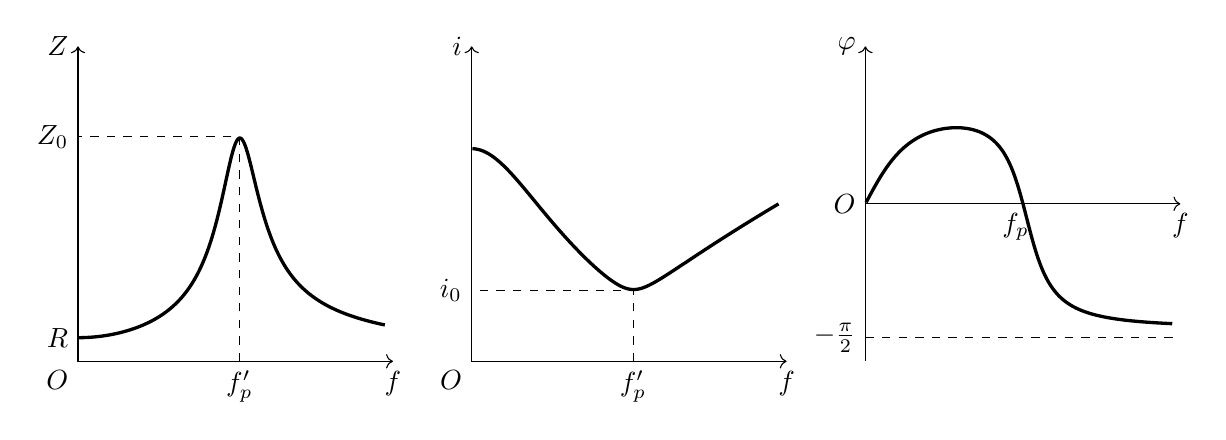
\begin{tikzpicture}
		\draw[<->] (0,4)node[left]{$ Z $}--(0,0)node[below left]{$ O $}--(4,0)node[below]{$ f $};
		\draw[very thick,domain=0.01:3.9,samples=1000] plot (\x,{0.6*sqrt((0.25+pow(0.5*\x,2))/(pow(1-0.235294*pow(\x,2),2)+pow(0.11765*\x,2)))});
		\draw[dashed] (2.05,0)node[below]{$ f_p' $}--(2.05,2.85)--(0,2.85)node[left]{$ Z_0 $};
		\node[left] at(0,0.3) {$ R $};
		
		\draw[<->] (5,4)node[left]{$ i $}--(5,0)node[below left]{$ O $}--(9,0)node[below]{$ f $};
		\draw[very thick,domain=5.01:8.9,samples=1000] plot (\x,{0.7+1/sqrt((0.25+pow(0.5*(\x-5),2))/(pow(1-0.235294*pow((\x-5),2),2)+pow(0.11765*(\x-5),2)))});
		\draw[dashed] (7.05,0)node[below]{$ f_p' $}--(7.05,0.90)--(5,0.9)node[left]{$ i_0 $};
		
		\draw[<-] (10,4)node[left]{$ \varphi $}--(10,0);
		\draw[very thick,domain=10.01:13.9,samples=1000] plot (\x,{2+rad(atan((\x-10-0.235*(\x-10)*(0.25+pow((\x-10),2)))/0.5))});
		\draw[->] (10,2)node[left]{$ O $}--(14,2)node[below]{$ f $};
		\node[below left] at(12.2,2) {$ f_p $};
		\draw[dashed] (10,0.3)node[left]{$ -\frac\pi2 $}--(14,0.3);
	\end{tikzpicture}
\end{document}